\documentclass[a4paper,10pt]{article}
\usepackage[utf8x]{inputenc}
\usepackage{amsfonts}
\usepackage{amsmath}
\usepackage{graphicx}

%opening
\title{Problem Set 4, STAT365/665}
\author{Girish Sastry}

\begin{document}

\maketitle

\section{Exercise 1}

We first simulate data in the same way as the example R code from class. There
are 1000 generated samples in the training set and 1000 samples in the test set.
There are five features and a binary classification vector. The two classes are
labeled as '0' or '1' in the data set. A plot of the data is in figure 1.

We first carry out model fitting with classification trees from the rpart
package in R. This is cross validated with 10 folds to determine the final error.
The same procedure is carried on both the test and training data sets. For
bagging, we make use of the adabag R package, which provides many useful bagging
functions. We carry out bagging with 10-fold cross validation. The computation
procedure followed was the same as the one described in the Bagging paper by
Friedman et. al. The misclassification errors obtained are as follows:

\begin{tabular}{l*{6}{c}r}
 Method		& Test Error & Training Error \\
 \hline
 Classification Trees	& $17.47\%$ & $17.10\%$ \\
 Bootstrapped Aggregated Trees 	& $12.02\%$ & $12.58\%$ \\
\end{tabular}

With bootstrap aggregation, we expect to obtain better variance with less overfitting.
We also obtain a better misclassification error in both the test and training
sets. Bootstrap aggregation works by selecting with replacement $m$ sets and producing
$m$ models for these sets and selecting the output by voting (for classification). 
So, it makes sense that bagging with the majority vote would give us better classification
on this problem. It is interesting to note the significant change in error in the bagging
trials versus the regular classification tree trials. Considering that this data set
is simulated with a certain model, this increase in performance may only hold for this 
model. 

\section{Exercise 2}
The data set for this Exercise is The Insurance Company Benchmark data set, which contains
informations on customers of an insurance company. This data set consists of 86 features.
These features contain information on product usage and sociodemographic data. We aim to 
classify the customers in two ways: either they would buy the insurance, or they would not.
This is a binary classification problem. 

We carry out tree based methods: a classic decision tree, random forest, and three variants
of the AdaBoost boosting algorithm: default AdaBoost, gentle AdaBoost, and L2 AdaBoost. The
ipred package in R was used for the decision tree. The randomForest package was used to carry
out random forests, and the ada stochastic boosting package was used for boosting. The errors
in both the training and test sets are as follows:

\begin{tabular}{l*{6}{c}r}
 Method		& Test Error & Training Error \\
 \hline
 Blind Prediction	& $5.95\%$ & $5.98\%$ \\
 Classic Decision Tree	& $5.95\%$ & $5.98\%$ \\
 Random Forests 	& $2.37\%$ & $2.60\%$ \\
 Default AdaBoost	& $5.95\%$ & $5.98\%$ \\
 Gentle AdaBoost	& $4.90\%$ & $5.00\%$ \\
 L2 AdaBoost		& $5.95\%$ & $5.96\%$ \\
\end{tabular}

We see that most of the errors across all the methods are pretty low. But, we have to be careful.
Because the data set has such a small number of positive classifications relative to the number
of samples, even the blind prediction gives training and test errors of less than 6\%. The
classic decision tree gives the same training and test errors as the blind prediction, and upon
closer inspection, we see that it just gives us the blind prediction (fig. 2). To improve these
results, we turn to random forests. Random forests give us better test and training errors, and
we see that the random forest model actually fits some data points in the ``1'' class (i.e. 
will buy the insurance) (fig. 3). This is encouraging, and perhaps this can be explained just
by the methodology of random forests. Because random forests work by running many trees on a
slightly perturbed data set, it gives better results. Intuitively, this makes sense given the 
nature of the data set -- there are so few positive classifications in the training set. A cursory
look at the weights used by the random forest algorithm shows that there are a few features that
have importance values of greater than 7: PBRAND (fire policies), PPERSAUT (car policies), and MOSTYPE (customer
subtype). This sheds some light on the types of people who would buy insurance, and it makes sense --
demanding fire policies or automobile policies would encourage buying of insurance. Similarly, customers
who are higher income should be more likely to buy insurance.

Boosting does not appear to provide any substantial gain in performance. All three of the boosting
methods we attempted provided similar results. The ``gentle'' AdaBoost was the best, but even so
it did not decrease the error rate by that much, and only assigned 14 positive classifications. It
appears that even boosting, which works by iteratively adding weak learnings to create a strong learning
classifier (based on variances), does not substantially improve over the blind prediction. From
these methods attempted, it appears that random forests provide the best results and the most information
about the type of customer that will purchase insurance.

\section{Appendix}

This section contains the figures referenced in the writeup and the R code used for the experiments.


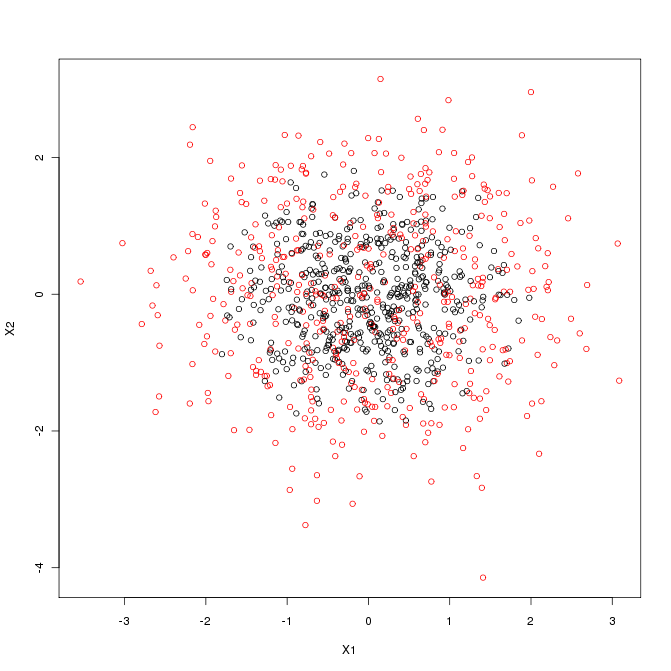
\includegraphics[width=100mm]{simulated_classes.png}

Figure 1: Simulated Data

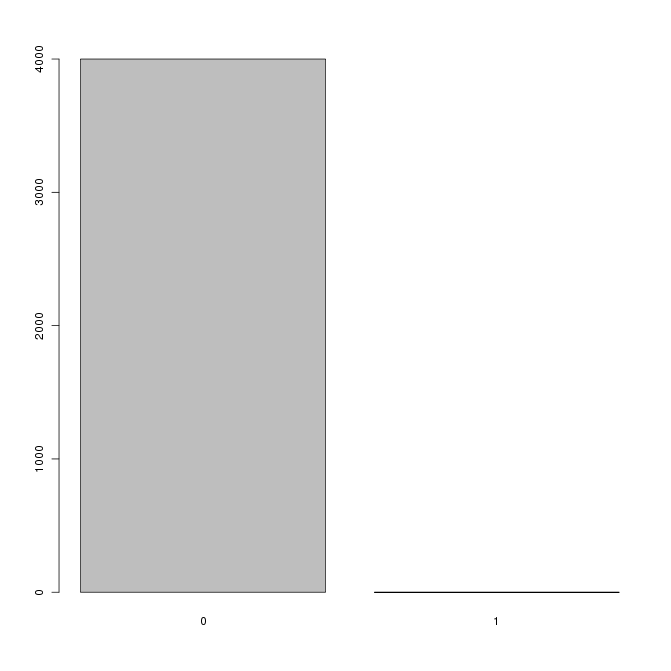
\includegraphics[width=100mm]{vs_blind.png}

Figure 2: Decision Tree Classification for Caravan Data



\includegraphics[width=100mm]{random_forest.png}

Figure 3: Random Forest Classification for Caravan Data
\end{document}
